\subsection{Three Consecutive Fast Intervals}
\label{sec:tcfi}
\begin{figure}[t]
	\centering
	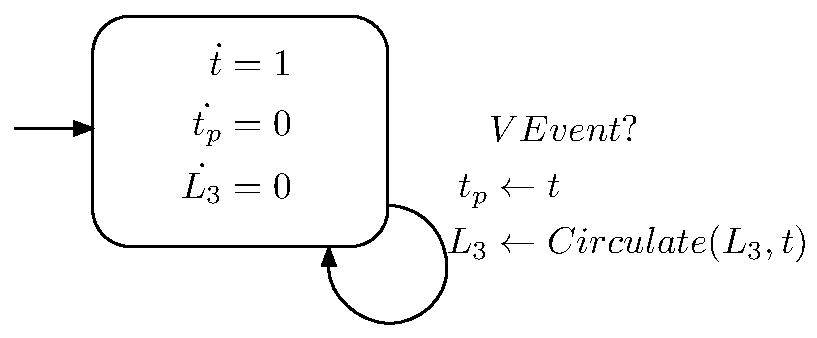
\includegraphics[scale=0.3]{figures/TCFI}
		\vspace{-10pt}
	\caption{Three Consecutive Fast Intervals $\Sys_{TCFI}$}
	\label{fig:tcfi}
\end{figure}
Our first module simply detects whether three consecutive fast intervals have occurred, where `fast' means the interval length, measured between 2 consecutive peaks on the \ac{EGM} signal, is shorter than some pre-set amount.
See Fig. \ref{fig:tcfi}.
States $t$ and $t_p$ are clocks as before.
The vector $L_3$ is three-dimensional, and stores the values of the last three intervals.
The event VEvent? is shorthand for the transition $y(t) \geq Th$ being taken by the $\Sys_{Sense}$ automaton.
In other words, it indicates a ventricular event.
Then $L_3$ gets reset to $L_3^+ = (z_1,z_2,z_3)^+ \defeq \text{Circulate}(L_3,t-t_p)$ where
\begin{equation}
L_3^+ = 
\left(\begin{matrix}
z_2\\z_3\\t-t_{p}\\
\end{matrix}
\right)
=
\left(\begin{matrix}
0 & 1 & 0\\0& 0& 1\\0& 0 &0
\end{matrix}
\right) L_3 + 
\left(\begin{matrix}
0\\0\\t-t_p
\end{matrix}
\right)
\end{equation}
%
\begin{lemma}
	$\Sys_{TCFI}$ is STORMED.
\end{lemma}
